\documentclass[12pt]{article}
\usepackage{amsmath}
\usepackage{graphicx}
\usepackage{subcaption}
\usepackage{hyperref}
\usepackage{url}
\usepackage{booktabs}
\usepackage{placeins}
\usepackage{pdflscape}
\usepackage{multirow}
\usepackage{color}
\usepackage[latin1]{inputenc}

% The following parameters seem to provide a reasonable page setup.
\topmargin 0.0cm
\oddsidemargin 0.2cm
\textwidth 16cm 
\textheight 21cm
\footskip 1.0cm

% Include your paper's title, authors and date here
\title{PHY 982 Homework 2}
\author{John Ash, Mengzhi Chen, Tong Li, Jason Surbrook}
\date{Feburary 27, 2018}

%%%%%%%%%%%%%%%%% END OF PREAMBLE %%%%%%%%%%%%%%%%

\begin{document}
\maketitle

\section{Elastic scattering calculations of a nucleon on $^{208}$Pb target} \label{part1}
\subsection{Coulomb scattering}
	In the case of point-Coulomb scattering, the Coulomb interaction between the projectile and the target with charges $Z_1$ and $Z_2$ is 
	\begin{equation}
		V_c(R)=\frac{Z_1Z_2e^2}{R^2},
	\end{equation}
	where R is the distance between them. The Schr\"{o}dinger's equation with this potential can be solved analytically. Related discussions are detailed in Ref.\cite{thompson2009nuclear}. In sum, the angular distribution of point-Coulomb potential is described by the differential cross section
	\begin{equation}\label{Ruther}
		\sigma(\theta)=\frac{\eta^2}{4k^2\sin^4(\theta/2)};\ \eta=\frac{Z_1Z_2e^2}{\hbar}\left(\frac{\mu}{2E}\right)^{\frac{1}{2}},
	\end{equation} 
	where $\mu$ is the reduced mass and $k$ is the wave number with the energy $E$. It worth noticing that the Eq. \ref{Ruther} is the same as the classical \emph{Rutherford cross section}.
	
	When the finite size of the target is included, due to different charge distributions, the interaction between the projectile and the target becomes more complicated. 
	
  	Normally, these potentials are not analytically solvable. Sometimes, we can apply the \emph{plane wave Born approximation} (PWBA) for the Coulomb scattering. Under PWBA, the differential cross section is 
  	\begin{equation}\label{ruther}
	\sigma(\theta)=\frac{\eta^2}{4k^2\sin^4(\theta/2)}\left|F(\theta)\right|^2,\end{equation}
	where $F(\theta)$ is called the \emph{form factor} related with the charge distribution as
	\begin{equation}\label{formfactor}
	F(\theta) = \int e^{i(\vec{k}_f-\vec{k}_i)\cdot\vec{r}'}\rho(r')d^3r'.
	\end{equation}
	
\subsection{Form factor of a solid sphere}
	To see substantial influence of the form factor, we give an simple example. 
	Suppose the charge distribution of the target with charge $Z_2$ is homogenous inside a solid sphere with radius $a$, which means
	\begin{align}
		\rho(R) &= \frac{3}{4\pi a^3}\ \rm{for}\ R<a\\
		&= 0\ \rm{elsewhere}.
	\end{align}
	The form factor is then calculated from Eq. \ref{formfactor}
	\begin{equation}\label{sphereformfactor}
		F(\theta)= \frac{3}{qa}\left(\frac{\sin(qa)}{(qa)^2}-\frac{\cos(qa)}{qa}\right) = \frac{3j_1(qa)}{qa}.
	\end{equation}
	where $j_1$ is spherical Bessel functions and $q=2k\sin(\theta/2)$. In Figure \ref{fig:formfactor}, we show the differential cross sections' ratio between these two cases. We can see fluctuation appears due to diffraction of finite-size body.

	 \begin{figure}[t]
		\centering
		\includegraphics[width=0.5\textwidth]{1_1.png}
		\caption{Differential cross sections for solid sphere charge distribution. Here we take $a=1;k=10$.  }
		\label{fig:formfactor}
	\end{figure}
	
  	In sum, we see the finite-size target can give cross sections different from the point-like case.
\subsection{Description of elastic scattering using optical potentials}
	In this section, we study the elastic scattering between nucleons and the $^{208}$Pb target with the help of FRESCO\cite{FRESCO} . Their effective interaction is referred to as the optical potential. We take the global parameterizations from Ref. \cite{capote2009ripl,koning2003local} as the input for FRESCO.
	
	In the first step, we take two lab energies 5 and 50 (40) MeV for proton (neutron) in our calculations. The results together with experimental data are shown in Figure \ref{fig:angulardistribution}. It gives the angular distributions in center of mass for protons and neutrons. For the 5 MeV proton, the curve agrees well with the \emph{Rutherford cross section}. Given that the radius parameter of optical potential is $r_w\sim1.2\ fm$, we can estimate the Coulomb barrier for a proton to overcome. It should be 
	\begin{equation}
	E_{Coul}\approx\frac{Z_1Z_2e^2}{r_w+R_2}\approx15\ \rm{MeV}.
	\end{equation}
	
	We can see that 5 Mev is much lower than the Coulomb barrier. Thus, this scattering can be referred as a point-like Coulomb scattering properly. The agreement with the \emph{Rutherford cross section} also verifies this point.
	For neutrons, there is no Coulomb interaction, hence the value of the neutron cross section being listed as $fm^2$. At 5 MeV the cross section hints at a broad diffraction pattern.
	
	Since 50 MeV is strong enough to overcome the Coulomb barrier, the effective interaction plays a role and induces a diffraction pattern in Figure \ref{fig:angulardistribution}. 
	The neutron cross section at 40 Mev exhibits a similar behavior, speaking to the dominance of the nuclear interaction at this energy.
	 We can also see that our curves basically obey same trends as experiments. 
	 However, they deviate in values, especially for neutron. 
	 It is because we use the global parameterizations. 
	 We will include the qualitative analyses and better fittings in the next section.
	  In order to explore the influence of the optical potential, we will keep using these energies in following calculations.
	
	\begin{figure}[t]
	\centering
	\includegraphics[width=0.92\textwidth]{5.png}
	\caption{Differential cross sections for nucleons scattering with $^{208}$Pb at 5 and 50MeV. Left panel is proton and right panel is neutron  }
	\label{fig:angulardistribution}
	\end{figure}
	
	In the next step, we would like to see the influences of the depth of optical potential's imaginary part of the S-matrix. 
	Fixing other parameters, we scale the depth of imaginary parts $V_i$ (including volume, surface derivative and spin-orbit potentials) a factor of 1.5, 0.5 and 0. 
	The modules of S-matrix for the proton and the neutron are shown in Table \ref{pSmatrix} and \ref{nSmatrix}. 
	
	We can see that as we lower the depth, $|\mathbf{S}|^2$ fluctuates and eventually converges to one which indicates an elastic scattering. It inspires us that the imaginary parts can describe absorptions in scattering processes. It also worth noticing the fluctuation of $|\mathbf{S}|^2$ with varying $V_i$ in each partial wave. For this reason, there is no simple monotonous relations between the relative depth $\bar{V}$ and the total absorptive cross section.

	\begin{table}[]
\centering
\begin{tabular}{cccccc}
\toprule
\toprule
\multicolumn{6}{c}{Proton partial waves}                                                                         \\
 \midrule
L                     & J                     & $|\mathbf{S}|^2$($\bar{V}$=1.5) & $|\mathbf{S}|^2$($\bar{V}$=1.0) & $|\mathbf{S}|^2$($\bar{V}$=0.5) & $|\mathbf{S}|^2$($\bar{V}$=0.0) \\
0                     & 0.5                   & 6.45E-04                     & 2.33E-04                     & 1.56E-02                     & 1.0                          \\
1                     & 0.5                   & 9.17E-04                     & 1.17E-03                     & 1.63E-02                     & 1.0                          \\
2                     & 1.5                   & 8.33E-04                     & 1.28E-04                     & 1.34E-02                     & 1.0                          \\
1                     & 1.5                   & 9.19E-04                     & 1.23E-03                     & 1.74E-02                     & 1.0                          \\
2                     & 2.5                   & 7.97E-04                     & 1.17E-04                     & 1.52E-02                     & 1.0                          \\
3                     & 2.5                   & 1.27E-03                     & 1.64E-03                     & 1.81E-02                     & 1.0                          \\
4                     & 3.5                   & 1.51E-03                     & 2.89E-04                     & 1.02E-02                     & 1.0                          \\
3                     & 3.5                   & 1.27E-03                     & 1.85E-03                     & 2.11E-02     
	& 1.0                          \\
   
$\cdots$           &$\cdots$                    & $\cdots$                            & $\cdots$                           & $\cdots$                           & $\cdots$                                                                \\
\bottomrule
\bottomrule
\end{tabular}
\caption{The modules of S-matrix for proton partial waves with varying imaginary potentials, where $\bar{V}$ is the scaled depth defined as $V_i(new)/V_i(initial)$.}
\label{pSmatrix}
\end{table}

\begin{table}[]
\centering
\begin{tabular}{cccccc}
\toprule
\toprule
\multicolumn{6}{c}{Neutron partial waves}                                                                         \\
 \midrule
L                     & J                     & $|\mathbf{S}|^2$($\bar{V}$=1.5) & $|\mathbf{S}|^2$($\bar{V}$=1.0) & $|\mathbf{S}|^2$($\bar{V}$=0.5) & $|\mathbf{S}|^2$($\bar{V}$=0.0) \\
0 & 0.5 & 7.88E-04                     & 1.40E-03                     & 2.16E-02                     & 1.0                            \\
1 & 0.5 & 5.24E-04                     & 4.68E-05                     & 1.75E-02                     & 1.0                            \\
2 & 1.5 & 8.94E-04                     & 1.62E-03                     & 2.29E-02                     & 1.0                            \\
1 & 1.5 & 5.24E-04                     & 4.68E-05                     & 1.75E-02                     & 1.0                            \\
2 & 2.5 & 8.94E-04                     & 1.62E-03                     & 2.29E-02                     & 1.0                            \\
3 & 2.5 & 7.27E-04                     & 1.66E-05                     & 1.67E-02                     & 1.0                            \\
4 & 3.5 & 1.15E-03                     & 1.87E-03                     & 2.51E-02                     & 1.0                            \\
3 & 3.5 & 7.27E-04                     & 1.66E-05                     & 1.67E-02                     & 1.0                            \\$\cdots$           &$\cdots$                    & $\cdots$                            & $\cdots$                           & $\cdots$                           & $\cdots$                                                                \\
\bottomrule
\bottomrule
\end{tabular}
\caption{The modules of S-matrix for neutron partial waves with varying imaginary potentials, where $\bar{V}$ is the scaled depth defined as $V_i(new)/V_i(initial)$.}
\label{nSmatrix}
\end{table}

    \begin{figure}[t]
		\centering
		\includegraphics[width=0.92\textwidth]{7.png}
		\caption{Differential cross sections for nucleons scattering with $^{208}$Pb with different radius parameters at 50MeV, where ratio is defined as $r_{new}/r_{initial}$. Left panel is proton and right panel is neutron.  }
		\label{fig:radiusparameter}
	\end{figure}

	Moreover, we are interested in the effects brought by different radius parameters. 
	In analogy with the Fresnel circular disk diffraction, as distance between disk and screen increases, the rings become denser.
	We can also check the special situation in Eq. \ref{sphereformfactor}, since $j_1(x)$ has fixed zero points, then, as radius parameter increases, we expect more compact diffraction patterns. 
	We don't scale the Coulomb interaction with optical potentials at same time, so we should see stronger up-down shift for proton caused by it.
	
	Again, fixing other parameters, we repeat our calculations by scaling the radius parameters $r$ (including volume, surface derivative and spin-orbit potentials) a factor of 0.2, 0.5, 2, 3 and 4. 
	The results are shown in Figure \ref{fig:radiusparameter}.
	For the proton, we observe a dramatic up-down shifts and denser diffraction patterns with increasing $r$. 
	It's the synergistic effect by the Coulomb and optical potentials. 
	As for neutron, the amplitude changing of pattern is relative small as it only feels the optical potential. 
	Although the interactions are more complicated than the solid sphere, the trends in these two figures agree well with our anticipations.
	
	The total reaction cross section and the absorptive cross section are equal in a single channel elastic scattering. For neutron, we extract them according to the equation
	\begin{equation}
		\sigma_{e}=\frac{\pi}{k^2}\sum_{J}(2J+1)(1-|\mathbf{S}_J|^2).
			\end{equation}
	The total reaction and absorptive cross sections are $3.764\times 10^3$ mb. The number deviates little from the value $3.796\times 10^3$ mb given directly by FRESCO for slightly different physical constants used.
	

\section{Fit optical potentials for elastic scattering of a nucleon on $^{208}$Pb target}
In this section we will do $\chi^2$ data fitting to obtain optical potentials 
for the elastic scattering of a proton or neutron on $^{208}$Pb. 
Experimental data are taken from Ref. \cite{MANI1971384_ProtonPb208Data} for proton and 
and \cite{PhysRevC.85.024619_NeutronPb208Data} for neutron. 
The beam energies of proton and neutron are 49.35 MeV and 40.0 MeV, respectively. 
In addition, we choose the optical parameters employed in Sec. \ref{part1} (Ref. \cite{capote2009ripl,koning2003local}) 
as the starting point of our fitting. 
All the results discussed in this section are generated by SFRESCO (Ref. \cite{FRESCO}). 

\subsection{Fit process and results}
All the intermediate and final results of our fitting are summarized in Table \ref{proton_table} (for proton) and Table \ref{neutron_table} (for neutron). 
For simplicity, we neglect spin-orbit components at the beginning, and only volume real and volume imaginary components are included. 
Keeping the volume imaginary component unchanged, we fit the volume real part (index 2 in Table \ref{proton_table} and \ref{neutron_table}), 
which cannot reduce $\chi^2/N$ to a low value. 
Then, we vary both volume real and imaginary parts simultaneously (index 3 in Table \ref{proton_table} and \ref{neutron_table}) and 
achieve a significant improvement.  
However, for proton the diffuseness parameter av becomes too small to be considered physical. 
\par
Another choice of optical potential is to use a surface imaginary component instead of a volume one. 
Starting from parametrization of index 4 in Table \ref{proton_table} and \ref{neutron_table}, we fit the volume real part and surface imaginary part 
(index 5 in Table \ref{proton_table} and \ref{neutron_table}). 
For both proton and neutron, a surface imaginary component gives a lower $\chi^2/N$, 
and thus we will add spin-orbit terms onto this optical potential form. 
\par
As shown in the last four lines in Table \ref{proton_table} and \ref{neutron_table}, 
we gradually add and fit different parameters in the spin-orbit term.  
As for proton, the description can hardly be improved by only adding a real spin-orbit potential (index 6 in Table \ref{proton_table}).  
If we only add a imaginary spin-orbit component, the diffuseness parameter ``awso" will become negative and thus unphysical 
(index 8 in Table \ref{proton_table}). 
If both real and imaginary components of spin-orbit potential are included, $\chi^2/N$ will slightly decrease from 4.860 to 3.611,
(index 9 in Table \ref{proton_table}). 
However, the relative errors of ``Vso" and ``Wso" are larger than 0.1, so they are not well constrained. 
Therefore, spin-orbit potentials are not important for the description of scattering of a proton on $^{208}$Pb. 
\par
As for neutron, we fit the spin-orbit term in a similar way. 
All the unphysical and unconstrained parameters are shown in Table \ref{neutron_table}. 
Since no significant improvement is seen from adding spin-orbit potentials and lots of parameters become unphysical or unconstrained 
in our fitting process, we think that the spin-orbit term is not important for the description of scattering of a neutron on $^{208}$Pb. 
Fig. \ref{fig:bothfit} shows the differential cross sections calculated from optical potential 5 
(volume real term + surface imaginary term), which are close to the experimental results. 
Thus, our fitting results are good enough to be employed in further calculations.  

\begin{landscape}
	\begin{table}[t]
		\centering
		\caption{Fitting results of scattering of a proton on $^{208}$Pb. The beam energy is 49.35 MeV. 
		The unit of Vv, Wv, Ws, Vso and Wso is MeV, and the unit of rv, av, rwv, awv, rws, aws, rvso, avso, rwso and awso is fm. 
	    Unphysical values are highlighted in red. Values that are not well constrained are highlighted in blue. 
        Fig. \ref{fig:proton_fit} gives the differential cross section for optical potential 5 (marked in bold). }
		\label{proton_table}
		\footnotesize
		\begin{tabular}{cccccccccccccccccc}
			\hline
			\hline
			Index & Fit from & Vv  & rv  & av  & Wv & rwv & awv  & Ws & rws & aws & Vso & rvso & avso & Wso & rwso & awso & $\chi^2/N$ \\
			\hline
			1     & -          & 67.2     & 1.244   & 0.646    & 16.6     & 1.244    & 0.646    & -        & -        & -        & -         & -         & -         & -         & -         & -        & 78.285   \\
			2     & 1          & 46.1     & 1.262   & 0.574    & 16.6     & 1.244    & 0.646    & -        & -        & -        & -         & -         & -         & -         & -         & -        & 27.134   \\
			3     & 2          & 44.6     & 1.254   & 1.87E-04 & 4.89     & 1.726    & 0.171    & -        & -        & -        & -         & -         & -         & -         & -         & -        & 5.479    \\
			4     & -          & 46.1     & 1.262   & 0.574    & -        & -        & -        & 19.5     & 1.246    & 0.615    & -         & -         & -         & -         & -         & -        & 11.335   \\
			\textbf{5}     & \textbf{4}          & \textbf{45.3}     & \textbf{1.229}   & \textbf{0.528}    & \textbf{-}        & \textbf{-}        & \textbf{-}        & \textbf{13.2}     & \textbf{1.295}    & \textbf{0.713}    & \textbf{-}         & \textbf{-}         & \textbf{-}         & \textbf{-}         & \textbf{-}         & \textbf{-}        & \textbf{4.860}    \\
			6     & 5          & 45.2     & 1.232   & 0.489    & -        & -        & -        & 12.7     & 1.295    & 0.732    & \color{blue}{0.14}     & \color{blue}{1.07}     & \color{blue}{0.55}     & -         & -         & -        & 4.838    \\
			7     & -          & 45.2     & 1.232   & 0.489    & -        & -        & -        & 12.7     & 1.295    & 0.732    & -         & -         & -         & -3.1    & 1.08      & 0.57     & 12.026   \\
			8     & 7          & 45.1     & 1.242   & 0.507    & -        & -        & -        & 12.0     & 1.279    & 0.748    & -         & -         & -         & -2.1     & 0.66     & \color{red}{-0.028}   & 4.068    \\
			9     & 7          & 45.2     & 1.276   & 0.540    & -        & -        & -        & 15.7     & 1.239    & 0.710    & \color{blue}{-6.9}     & 0.84    & 0.55  & \color{blue}{-8.0}  & 1.03  & 0.53     & 3.661   \\
			\hline
			\hline
		\end{tabular}
	\end{table}

\begin{table}[b]
	\centering
	\caption{Fitting results of scattering of a neutron on $^{208}$Pb. The beam energy is 40.0 MeV. 
			The unit of Vv, Wv, Ws, Vso and Wso is MeV, and the unit of rv, av, rwv, awv, rws, aws, rvso, avso, rwso and awso is fm. 
			Unphysical values are highlighted in red. Values that are not well constrained are highlighted in blue. 
     		Fig. \ref{fig:neutron_fit} gives the differential cross section for optical potential 5 (marked in bold). }
	\label{neutron_table}
	\footnotesize
	\begin{tabular}{cccccccccccccccccc}
		\hline
		\hline
		index & Fit from & Vv   & rv    & av    & Wv    & rwv   & awv   & Ws   & rws   & aws   & Vso & rvso  & avso & Wso   & rwso & aso  & $\chi^2/N$ \\
		\hline
		1     & -        & 50.6 & 1.244 & 0.646 & 15.6  & 1.244 & 0.646 & -    & -     & -     & -   & -     & -    & -     & -    & -    & 261.394    \\
		2     & 1        & 40.3 & 1.245 & 0.903 & 15.6  & 1.244 & 0.646 & -    & -     & -     & -   & -     & -    & -     & -    & -    & 46.553     \\
		3     & 2        & 41.9 & 1.154 & 0.762 & 6.598 & 1.383 & 0.824 & -    & -     & -     & -   & -     & -    & -     & -    & -    & 7.900      \\
		4     & -        & 40.3 & 1.245 & 0.903 & -     & -     & -     & 13.8 & 1.246 & 0.510 & -   & -     & -    & -     & -    & -    & 98.423     \\
		\textbf{5}     & \textbf{4}        & \textbf{36.4} & \textbf{1.269} & \textbf{0.585} & \textbf{-}     & \textbf{-}     & \textbf{-}     & \textbf{14.4} & \textbf{1.097} & \textbf{0.500} & \textbf{-}   & \textbf{-}     & \textbf{-}    & \textbf{-}     & \textbf{-}    & \textbf{-}    & \textbf{4.638}      \\
		6     & 5        & 36.1 & 1.277 & 0.578 & -     & -     & -     & 15.7 & 1.108 & 0.498 & 8.3 & \color{red}{-4.3} & 3.2 & -     & -    & -    & 3.084      \\
		7     & -        & 36.4 & 1.269 & 0.585 & -     & -     & -     & 14.4 & 1.097 & 0.500 & -   & -     & -    & -3.1 & 1.08 & 0.57 & 35.163     \\
		8     & 7        & 36.4 & 1.273 & 0.593 & -     & -     & -     & 15.2 & 1.109 & 0.519 & -   & -     & -    & \color{blue}{-3.1} & 1.09 & 0.43 & 3.310      \\
		9     & 8        & 35.8 & 1.266 & 0.592 & -     & -     & -     & 14.9 & 1.107 & 0.513 & 4.9 & \color{red}{1.03}  & \color{red}{1.23} & -3.0 & 1.06 & 0.81 & 2.258      \\
		\hline
		\hline
	\end{tabular}
\end{table}
\end{landscape}
\begin{figure}[tb]
	\begin{subfigure}[tb]{0.5\textwidth}
		\centering
		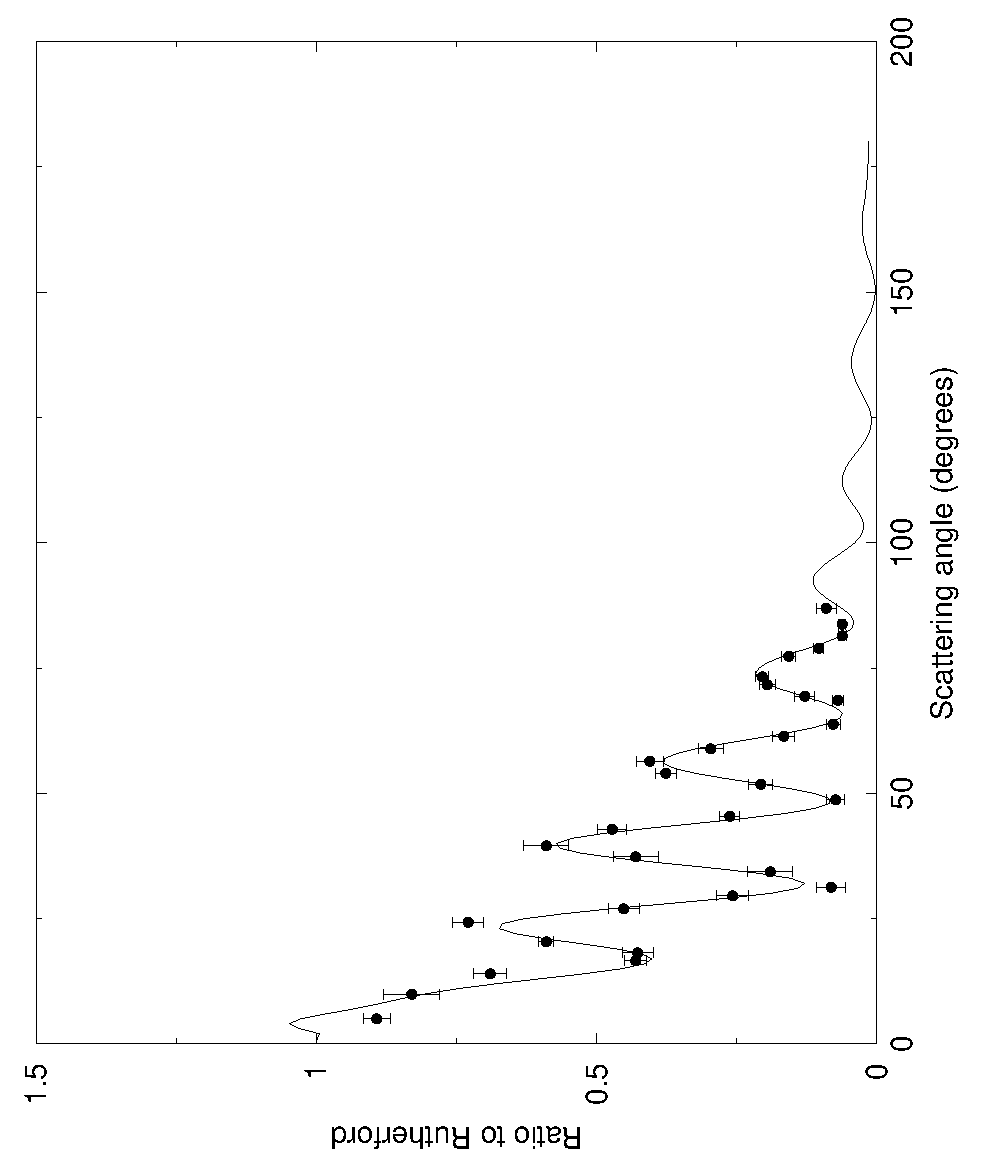
\includegraphics[width=0.65\textwidth,angle=270]{proton_fit.eps}
		\caption{Differential cross section of scattering of a proton on $^{208}$Pb with beam energy 49.35 MeV. 
		Optical potential 5 in Table \ref{proton_table} is used for the calculation. }
		\label{fig:proton_fit}
	\end{subfigure}
~
	\begin{subfigure}[tb]{0.5\textwidth}
		\centering
		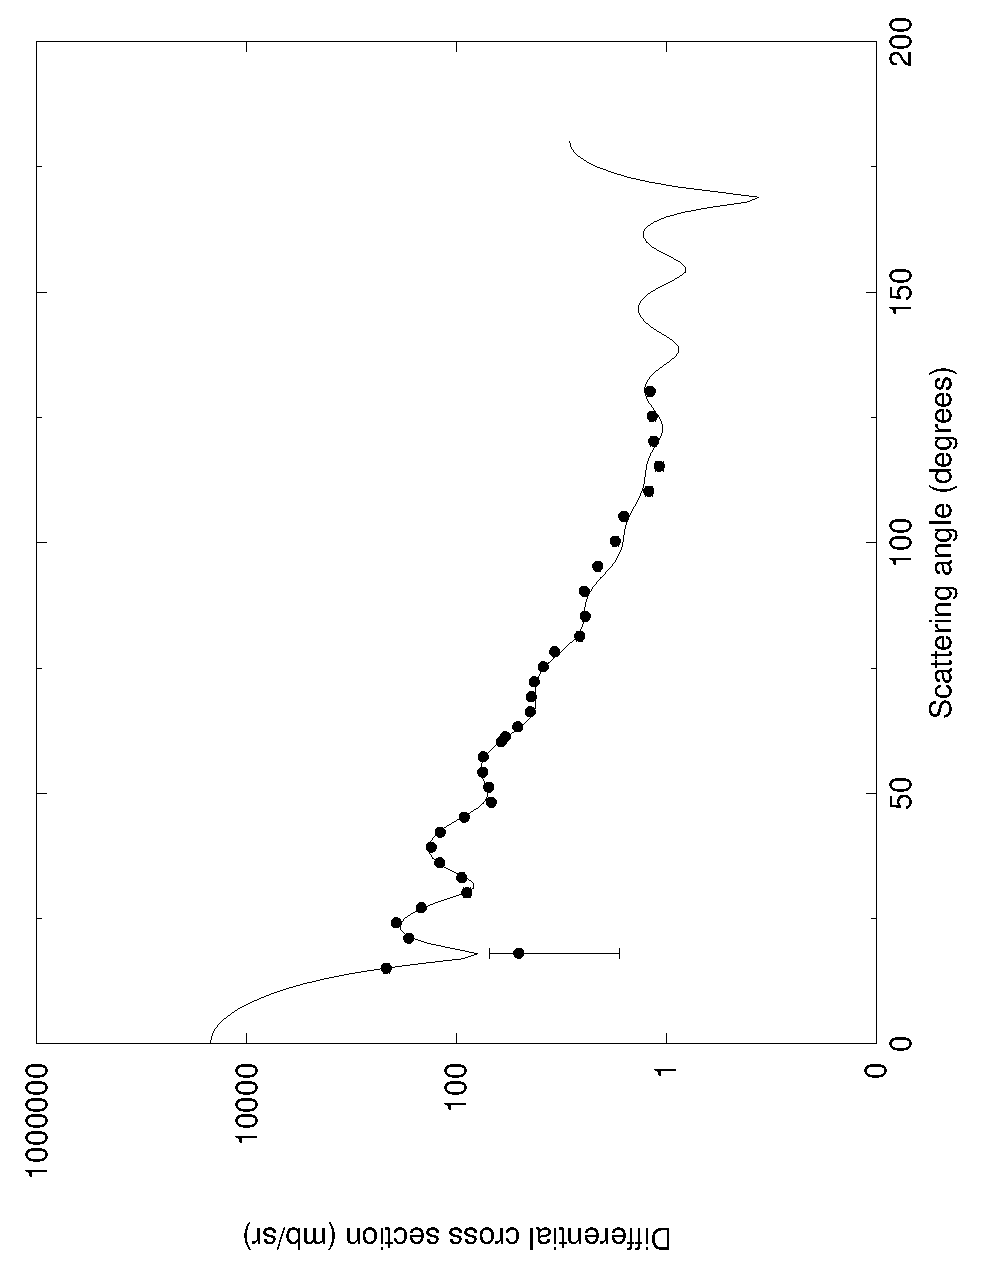
\includegraphics[width=0.65\textwidth,angle=270]{neutron_fit.eps}
		\caption{Differential cross section of scattering of a neutron on $^{208}$Pb with beam energy 40.0 MeV. 
			Optical potential 5 in Table \ref{neutron_table} is used for the calculation. }
		\label{fig:neutron_fit}
	\end{subfigure}
	\caption{Comparison of differential cross sections with experimental results. }
	\label{fig:bothfit}
\end{figure}

\subsection{Fit Sensitivity to Initialization}
Here we study the sensitivity of SFRESCO fitting to initial parameters. We used volume real and surface imaginary components of the optical potential only. Although there is improvement in the neutron scattering fit by inclusion of a spin-orbit imaginary term, optimal fits without this term are roughly 40\% of the fit with this additional term ($\chi^2/N = 3.310, 4.638 $). Optimal initial parameters were determined by successive fitting and reinitializing output parameters until a stable minimum was achieved with parameters comparable to the initial global potential fits from \cite{capote2009ripl}.
\par
In Figure \ref{fig:initializations} below, we plot the SFRESCO $\chi^2/N$ fit error against modifications of a single parameterization. To overlay dissimilar parameter values, the plotted input parameter is normalized by its determined optimized value. $\chi^2/N$ as a choice of parameter of interest (as opposed to the output value of the varied parameter) was from the observation that  $\chi^2/N$ correlates strongly with optical potential parameters approaching the optimal fit values within a few percent. From Fig \ref{fig:pnV}, we see that initializations to both depth parameters for protons and neutrons arrive at optimum for roughly $\pm$50\% of optimal values. From Fig. \ref{fig:pnr}, While not as centered around $\frac{P_{in}}{P_{optimal}}=1$ as the depth parameters, the radius parameters appear to converge for roughly $\pm$25\% of optimal values. In Fig. \ref{fig:pna}, we demonstrate that diffuseness is potentially the most convergent parameter (see neutron surface imaginary converge for $\pm$100\% of the optimal value), diffuseness is the least consistent parameter. The worst demonstrated convergence is the proton surface imaginary diffuseness, which converges for $\frac{P_{in}}{P_{optimal}}=1.0-0.0+0.5$.
\par
Two peculiarities were discovered while spanning these parameters.
\begin{enumerate}
	\item Multiple initializations regions of the proton real volume depth lead to optimal parameterization. Fig. \ref{fig:pnV} shows how $V_0\approx 0$ gives results consistent with $V_0 \approx V_{optimal}$ while the region $0.1 \leq \frac{V_0}{V_{optimal}} \leq 0.6$ returns a significantly worse fit.
	\item See the neutron real volume depth $\frac{V_0}{V_{optimal}} = 0.55 \pm <0.05$. This region of poorer $\chi^2$ metric sits in a narrow region ($<$ 3 MeV) of more optimal parameter finding. Given the approximate nature of the global potentials that served to set the parameter initializations, it is believable that a global parameterization based initialization could find a non-optimal local minima. So, we emphasize the value of repeated, varied initialization over a range deemed possible for a parameter.  
\end{enumerate}
\begin{figure}[h]
	\begin{subfigure}{0.5\textwidth}
		
		\centering
		\includegraphics[width=0.98\textwidth]{pnV.png}
		\caption{Optical potential depth parameters }
		\label{fig:pnV}
	\end{subfigure}
	\begin{subfigure}{0.5\textwidth}
		\centering
		\includegraphics[width=0.98\textwidth]{pnr.png}
		\caption{Nuclear radius parameters }
		\label{fig:pnr}
	\end{subfigure}
	\begin{subfigure}{0.5\textwidth}
		\centering
		\includegraphics[width=0.98\textwidth]{pna.png}
		\caption{Nuclear diffuseness parameters  }
		\label{fig:pna}
	\end{subfigure}
	\caption{Measure of error of SFRESCO fits for different initial parameterization of the depth part of the optical potential for 49.35 MeV protons ($\pi$) and 40 MeV neutrons ($\nu$) scattering on $^{208}$Pb. Plotted on the x-axis is the ratio of $\frac{P_{initial}}{P_{optimal}}$. }
	\label{fig:initializations}
\end{figure}

\bibliographystyle{unsrt}
\bibliography{references}
\end{document}